% !TeX root = ../main.tex

\chapter{Hardware}\label{chapter:Hardware}

This chapter gives an overview of hardware used to implement this thesis. In addition to the basic set of \textit{HTC Vive} hardware consisting of two base stations, a headset and two \glspl{controllergl},  three \textit{Vive Trackers} are used to track the user's feet and his upper torso. It is a \gls{vra} system jointly developed by \textit{HTC} and \textit{Valve Corporation} \autocite{htcValveVive}. The consumer version was released on the 7th of June 2016 at a price of \$799 US \autocite{htcShip}.


\section{Base Stations}

The base stations, also called Lighthouses, are placed diagonally apart and ideally above head height around the designated tracked area, which can be up to 3.5m by 3.5m \autocite{viveProductPage}. They are connected wirelessly to the computer and emit timed infrared light pulses 60 times per second, which are registered by tracked objects in order to calculate their position and pose in the tracked area \autocite{lighthouseHowWork}.
\begin{figure}[h]
    \centering
    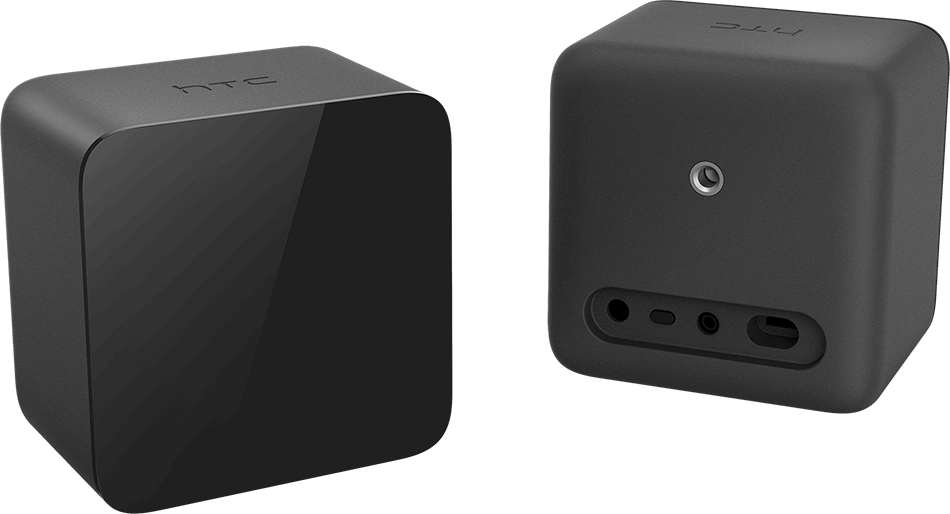
\includegraphics[height=0.2\textheight]{figures/vive-hardware-base-stations.png}
    \caption{Base Stations, also called Lighthouses \autocite{viveProductPage}}
    \label{fig:lighthouse}
\end{figure}


\section{Headset}

The headset is a \gls{hmda} with two AMOLED 3.6" panels with a resolution of 1080 by 1200 pixels each per eye, running at a refresh rate of 90Hz. It allows users to see a field of view of about 110 degrees. 
\newline
There are many infrared sensors dotted around the casing, which detect infrared light pulses sent out from the base stations \autocite{lighthouseHowWork}. It also includes an accelerometer and a gyroscope, as well as a front facing camera \autocite{viveProductPage}. Data from these sensors is combined to calculate at high precision the headset's current position within the tracked area.
\newline
The headset is tethered to the computer by a collection of cables, carrying power as well as image, audio and other data. It offers a 3.5mm headphone jack to plug headphones into, as well as a USB port to attach other peripherals.
\begin{figure}[h]
    \centering
    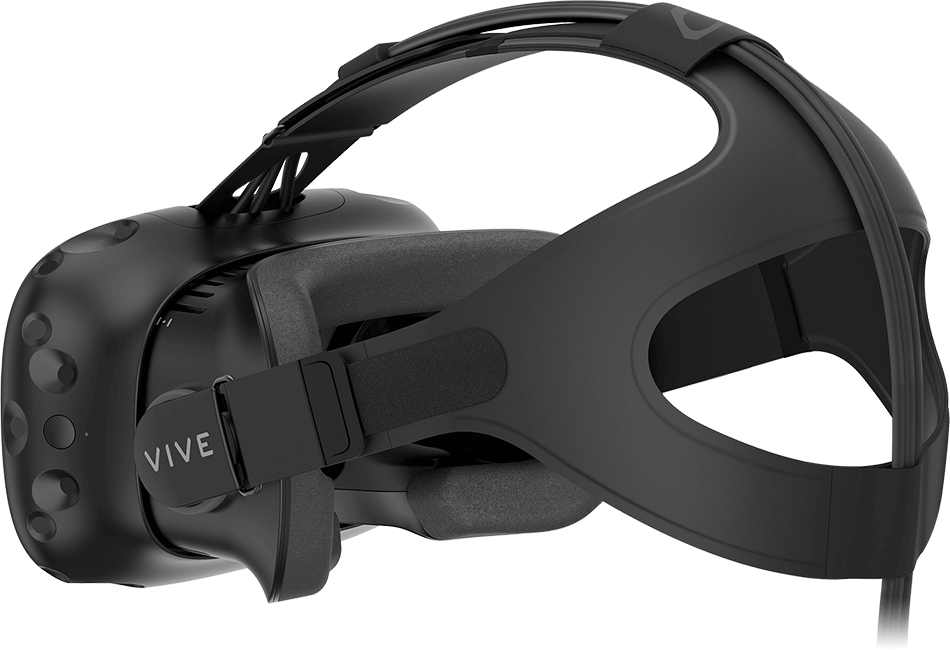
\includegraphics[height=0.2\textheight]{figures/vive-hardware-hmd-1}
    \caption{HTC Vive Headset \autocite{viveProductPage}}
    \label{fig:headset}
\end{figure}


\section{Controllers}
The \glspl{controllergl} use the same mechanisms as the headset to track their position. They are battery powered and connect wirelessly to the computer. Various input modalities are present on the \glspl{controllergl} which can be accessed by the \gls{vra} application \autocite{viveProductPage}:
\begin{itemize}
    \item Multifunctional trackpad
    \item Grip buttons
    \item Dual-stage trigger
    \item Menu button
\end{itemize}
A vibration motor is included, which can also be controlled by the \gls{vra} application, in order to, for example, provide haptic feedback.
\begin{figure}[h]
    \centering
    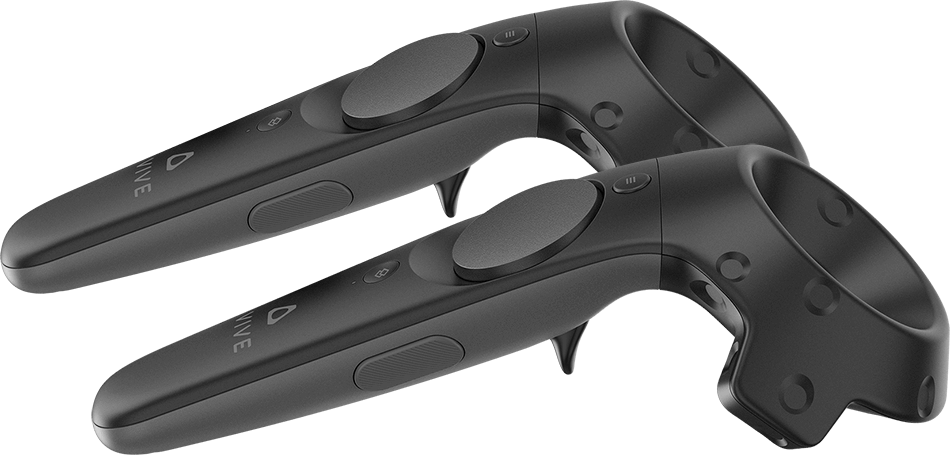
\includegraphics[height=0.2\textheight]{figures/vive-hardware-controllers-1}
    \caption{HTC Vive Controllers \autocite{viveProductPage}}
    \label{fig:controllers}
\end{figure}


\section{Trackers}
The \textit{Vive Trackers} are a separately sold motion tracking accessory, intended to be attached to other physical accessories, such as guns or swords, or strapped to body parts for full body tracking. They became widely available for consumers by the end of 2017 \autocite{viveTrackerLaunch}.
\newline
Their position is tracked the same way as the controllers and headset. They also connect wirelessly to the computer and are battery powered. No input modalities intended to be accessed by a \gls{vra} application are included, however on the underside is a connector which offers 6 electrical pins, called \textit{Pogo pins}. These can be used to communicate with the attached accessory. In the centre on the underside is a standard camera mount, which is used to fasten the tracker to physical accessories or straps \autocite{viveTrackerDevGuide}.
\newline
The \textit{Vive Tracker} unfortunately does not include a vibration motor, relying instead on potential accessories to provide haptic feedback, however it can receive the instruction to vibrate like the controller, upon which \enquote{the POGO OUT pin sets an output of HIGH with the duration in ‘ms’} \autocite[p. ~29]{viveTrackerDevGuide}, so as long as the accessory supports it, the \textit{Vive Tracker} can be treated like the controller for haptic events.
\begin{figure}[h]
    \centering
    \subfloat[HTC Vive Tracker  \autocite{viveAccessoryPage}]{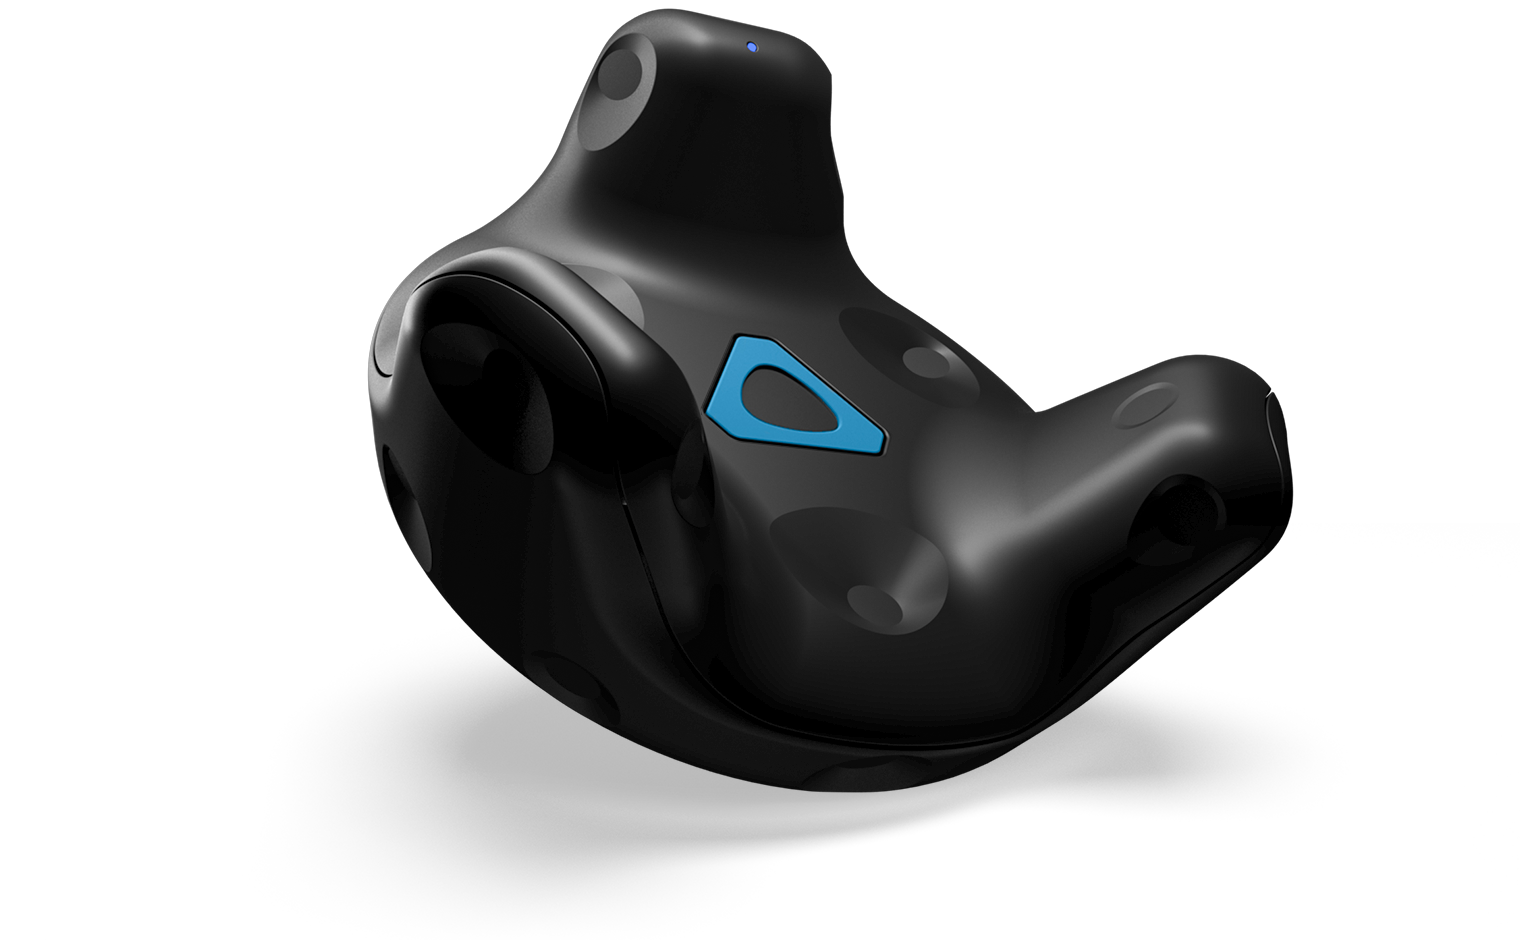
\includegraphics[width=0.4\textwidth]{figures/vive-tracker_2018_listing}}
    \hfill
    \subfloat[Mounted on Sword accessory \autocite{viveTrackerDevGuide}]{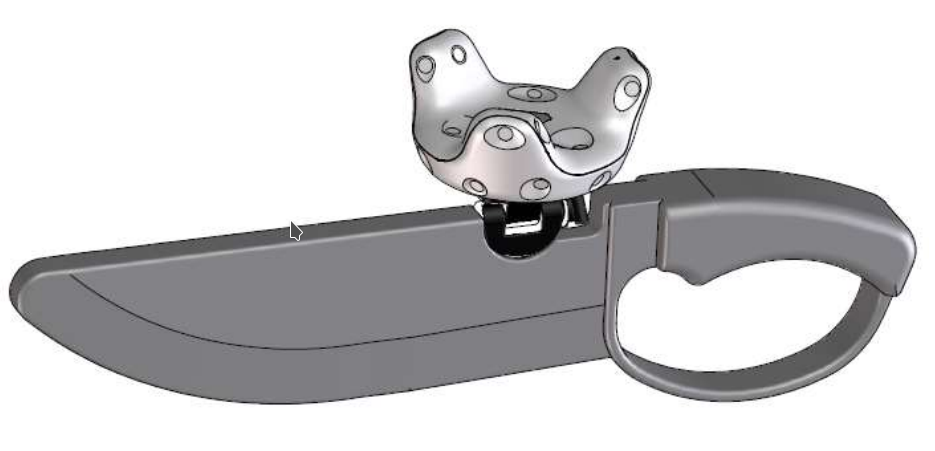
\includegraphics[width=0.3\textwidth]{figures/viveTrackerSword}}
    \hfill
    \subfloat[Attached to straps \autocite{viveTrackerDevGuide}]{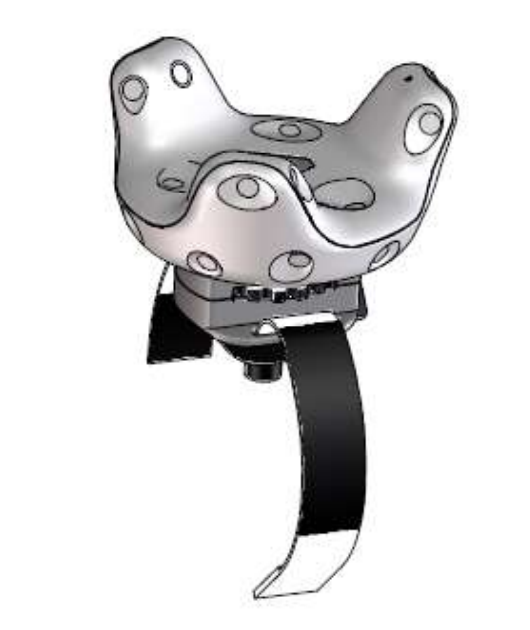
\includegraphics[width=0.2\textwidth]{figures/viveTrackerStrap}}
    \caption{HTC Vive Tracker}
    \label{fig:tracker}
\end{figure}